\documentclass[a4paper]{article}
\usepackage{color}
\usepackage{url}
\usepackage[T2A]{fontenc} % enable Cyrillic fonts
\usepackage[utf8]{inputenc} % make weird characters work
\usepackage{graphicx}
\usepackage[english,serbian]{babel}
\usepackage[unicode]{hyperref}
\hypersetup{colorlinks,citecolor=green,filecolor=green,linkcolor=blue,urlcolor=blue}
\newtheorem{primer}{Primer}[section]
\begin{document}
\title{DALL-E 2 - OpenAI\\ \small{Seminarski rad u okviru kursa\\Tehničko i naučno pisanje\\ Matematički fakultet}}
\author{Ognjen Marković\\ \small{ognjen.mark03@gmail.com}\\ Matija Milovanović\\ \small{matija.milovanovic55@gmail.com}\\ Bogdan Milovanović\\ \small{bogdan.milovanovic1106@gmail.com}\\ Bojana Radovanović\\ \small{bojanaradovanovic080@gmail.com} }
\date{11.~novembar 2022.}
\maketitle
\abstract{
DALL-E I DALL-E 2 su modeli mašinskog učenja koje je razvio OpenAI za generisanje digitalnih
slika pomocu tekstualnih opisa generisanih metodama obrade prirodnih jezika (eng. Natural language procesing - NLP). DALL-E je prvi put
spomenut na blogu OpenAI-a u januaru 2021. godine i tada je koristio verziju GPT-3 modifikovanu za
generisanje slika. U aprilu 2022. godine OpenAI je najavio DALL-E 2, naslednika dizajniranog da
generiše realističnije slike u višim rezolucijama koje mogu kombinovati koncepte, atribute i
stilove.}
\tableofcontents
\newpage
\section{Uvod}
\label{sec:uvod}
OpenAI je istraživačka laboratorija za veštačku inteligenciju (eng. Artificial Intelligence - AI) koju čine profitna korporacija OpenAI LP i njena matična kompanija, neprofitna OpenAI Inc. Kompanija, koja se smatra konkurentom DeepMind-u\footnote{DeepMind je kompanija koja uz pomoć veštačke inteligencije kreira programe koji koriste duboke neuronske mreže da bi naučili sebe kako da igraju različite igre kao što su Go i šah. Osnovana je 2010. godine, a već 2014. godine je kupljena od strane Google-a.}, sprovodi istraživanja u oblasti veštačke inteligencije sa navedenim ciljem promovisanja i razvoja prijateljske veštačke inteligencije na način koji koristi čovečanstvu u celini. Organizaciju su osnovali u San Francisku krajem 2015. godine Ilon Mask, Sem Altman i drugi, koji su zajednički obećali milijardu dolara. Mask je podneo ostavku na mestu u odboru u februaru 2018. godine, ali je ostao donator. U 2019. godini, OpenAI LP je od Microsoft-a dobio investiciju od milijardu dolara. Neki naučnici, poput Stivena Hokinga i Stjuarta Rasela, izrazili su zabrinutost da ako napredna veštačka inteligencija jednog dana dobije sposobnost da se redizajnira sve većom brzinom, nezaustavljiva „eksplozija inteligencije“ može dovesti do izumiranja ljudi. Mask karakteriše veštačku inteligenciju kao „najveću egzistencijalnu pretnju čovečanstva“. Osnivači OpenAI su je strukturisali kao neprofitnu organizaciju kako bi mogli da fokusiraju svoje istraživanje na stvaranjepozitivnog dugoročnog uticaja na ljude\cite{1}.
\section{Veštačka inteligencija}
\label{Veštačka inteligencija}
Veštačka inteligencija jedna je od retkih oblasti nauke o kojoj skoro svi, i eksperti, i oni koji to nisu, imaju neki stav. Neko smatra da ona donosi velike koristi, neko smatra da od nje prete opasnosti, a neko veruje i u jedno i u drugo. Neobično je onda da, s druge strane, ne postoji opšta saglasnost o tome šta je uopšte veštačka inteligencija i čime se ona bavi. Pod inteligencijom se obično podrazumeva sposobnost usvajanja, pamćenja i obrade određenih znanja. Iako postoji i shvatanje po kojem je centralni cilj veštačke inteligencije oponašanje ljudske inteligencije, većina podoblasti veštačke inteligencije ima drugačiji cilj. Obično je to rešavanje problema u kojima se javlja kombinatorna eksplozija, tj. u kojima je broj mogućnosti toliko veliki da se ne može sistematično ispitati u razumnom vremenu. Najveći deo zadataka veštačke inteligencije može se opisati u terminima algoritmike, pretrage, deduktivnog i induktivnog zaključivanja, i drugih preciznih matematičkih pojmova. Tek mali deo istraživača bavi se metodama koje pretenduju da dostignu opšte rasuđivanje u stilu čoveka. Veštačka inteligencija sastoji se od više podoblasti, naizgled slabo povezanih svojim sadržajem. Pitanje je onda šta je to zajedničko za njih, sem to što se uglavnom sve bave problemima u kojima se javlja mnoštvo mogućnosti koje se ne mogu ispitati sistematičnom pretragom. Termin "veštačka inteligencija" je ranije korišcén za opisivanje mašina koje oponašaju i prikazuju ljudske kognitivne veštine koje su povezane sa ljudskim umom, kao što su učenje i rešavanje problema. Ovu definiciju su od tada odbacili glavni istraživači AI koji sada opisuju AI u smislu racionalnosti i racionalnog delovanja, što ne ograničava način na koji se inteligencija može artikulisati.
\newpage
Primena veštačke inteligencije je jako široka i ona uključuje napredne veb pretraživače (npr. Google), sisteme za preporuke (koje koriste YouTube, Amazon i Netflix), razumevanje ljudskog govora (kao što su Siri i Alexa), automobile koji se samostalno voze (npr. Tesla), automatizovano donošenje odluka i takmičenje na najvišem nivou u sistemima strateških igara (kao što su šah i Go). Kako mašine postaju sve sposobnije, zadaci za koje se smatra da zahtevaju „inteligenciju“ često se uklanjaju iz definicije veštačke inteligencije.

Takođe prisutna je još jedna oblast veštačke inteligencije koje će nama biti jako interesantna, a to je NLP. Ona se bavi interakcijom između računara i ljudskog jezika, posebno kako programirati računare da obrađuju i analiziraju velike količine teksta na prirodnom jeziku. Cilj NLP-a je da kompjuter razume sadržaj dokumenata, uključujući kontekstualne nijanse jezika u njima. Tehnologija tada može precizno da izdvoji informacije  sadržane u dokumentima, kao i da kategorizuje i organizuje same dokumente\cite{2}.
\section{DALL-E 2}
\label{DALLE2}
\subsection{Tehnologija}
\label{subsec:tehnologija}
Model generativnog unapred obučenog transformatora (eng. Generative Pretrained Transformer - GPT) je prvobitno razvio OpenAI 2018. godine, koristeć arhitekturu transformatora. Prva iteracija, GPT, je unapređena da bi proizvela GPT-2 2019. godine. Godine 2020. ponovo je unapređena da bi proizvela GPT-3, sa 175 milijardi parametara. DALL-E-ov model je multimodalna implementacija GPT-3 sa 12 milijardi parametara koji „zamenjuje tekst za piksele“, obučen na parovima tekst-slika sa Interneta. DALL-E 2 koristi 3,5 milijardi parametara, što je manji broj od svog prethodnika.
\begin{table}[h!]
\begin{center}
\caption{U tabeli \ref{tab:tabela1} je prikazan hronološki razvitak DALL-E 2.} 
\vspace{0.5cm}
\begin{tabular}{|c|c|c|c|c|} \hline
2018&2019&2020&2021&2022\\ \hline
GPT&GPT-2&GPT-3 &DALL-E&DALL-E 2\\ \hline
\end{tabular}
\label{tab:tabela1}
\end{center}
\end{table}
Naziv softvera je sastavni deo imena animiranog robota Pikar lika VALL-E i španskog
nadrealističkog umetnika Salvadora Dalija. DALL-E 2 je razvijen i objavljen javnosti u saradnji sa CLIP-om (eng. Contrastive Language-Image Pre-Training - CLIP). Njegova uloga je da „razume i rangira“ sliku koja je izlaz iz DALL-E 
 predviđanjem koji je naslov sa liste od 32.768 naslova nasumično odabranih iz skupa podataka (od kojih je jedan bio tačan odgovor) najprikladniji za sliku. Ovaj model se koristi za filtriranje veće početne liste slika koje generiše DALL-E da bi se odabrali najprikladniji rezultati. Kad bismo pojednostavili stvari, ovaj model funkcioniše tako što počinje sa slikom koja se sastoji od nasumičnih piksela („šum“) i postepeno „uklanja šum“ slike. Tokom procesa uklanjanja
šuma, on se približava slici koja odgovara početnom izvornom tekstu koji je dat na ulazu.

\newpage

\subsection{Mogućnosti}
\label{subsec:mogućnosti}

DALL-E 2 može da:
\begin{itemize}
\item generiše slike u više stilova, uključujući fotorealistične slike i emotikone
\item da manipuliše i preuređuje objekte na svojim slikama
\item ispravno postavi elemente dizajna u nove kompozicije bez eksplicitnih instrukcija
\end{itemize}

Thom Dunn koji je pisao za BoingBoing je primetio da, na primer, "kada se zamoli da nacrta daikon rotkvu kako duva nos, pijucka kafu ili se vozi monociklom, DALL-E često crta maramicu, ruke i stopala na uverljivim mestima". DALL-E je pokazao sposobnost da „popuni prazna mesta“ kako bi zaključio odgovarajuće detalje bez specifičnih napomena kao što je dodavanje božićnih slika uputstvima koja se obično povezuju sa proslavom, i odgovarajuće postavljene senke slikama koje ih ne pominju. Šta više, DALL-E pokazuje široko razumevanje vizuelnih idizajnerskih trendova\cite{3}.

DALL-E je u stanju da proizvede slike za širok spektar proizvoljnih opisa sa različitih gledišta uz minimalan procenat grešaka. Mark Ridl, vanredni professor na Tehničkoj školi za interaktivno računarstvo u Džordžiji, otkrio je da DALL-E može da kombinuje koncepte (opisan kao ključni element ljudske kreativnosti) i ima sposobnost vizuelnog rasuđivanja dovoljnu da reši Rejvenove matrice (vizuelni testovi koji se često primenjuju ljudima za merenje inteligencije).

DALL-E 2 može da kreira veoma realistične slike kao npr. prikazan  portret basketa (slika \ref{fig:pas}.).
\begin{nesto1}
\begin{figure}[h!]
\begin{center}
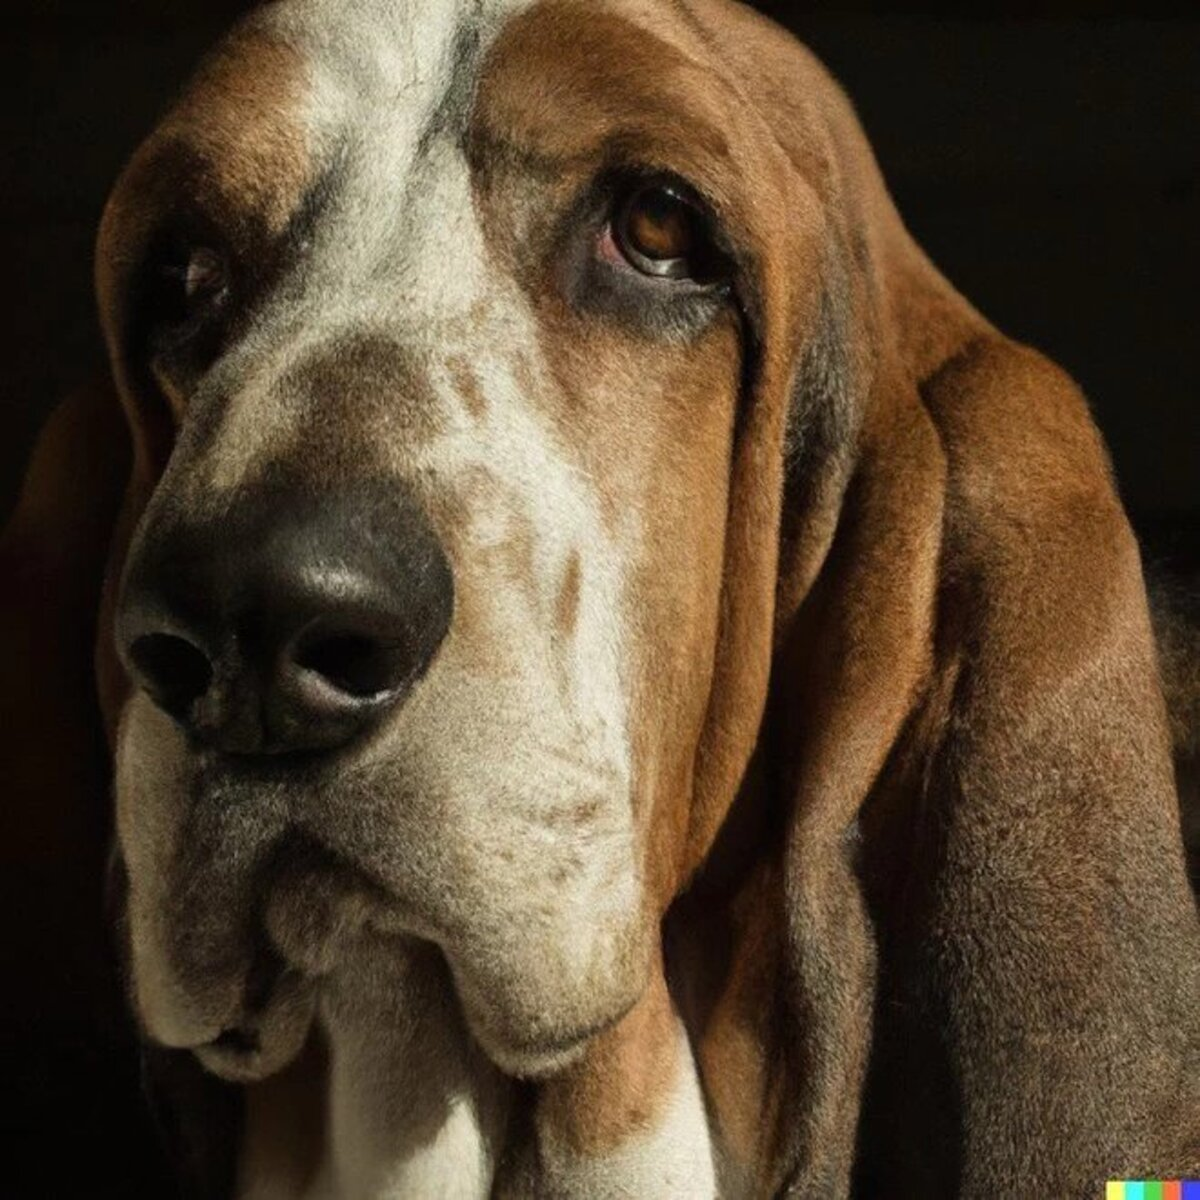
\includegraphics[scale=0.09]{pas.jpg}
\end{center}
\caption{Pas}
\label{fig:pas}
\end{figure}

Ali trik u svemu ovome je što ovaj pas ne postoji... Ova slika psa nije nastala tako što je osoba slikala svog četvoronožnpg prijatelja, već je slika koju je napravilo DALL-E 2. Takođe, u stanju je da kreira veoma realistične slike ljudi npr. prikaz  realne fotografije mlade žene plavih očiju i plave kose (slika \ref{fig:zena}.) ,kao i objekte koji u stvarnosti ne postoje.

\begin{figure}[h!]
\begin{center}
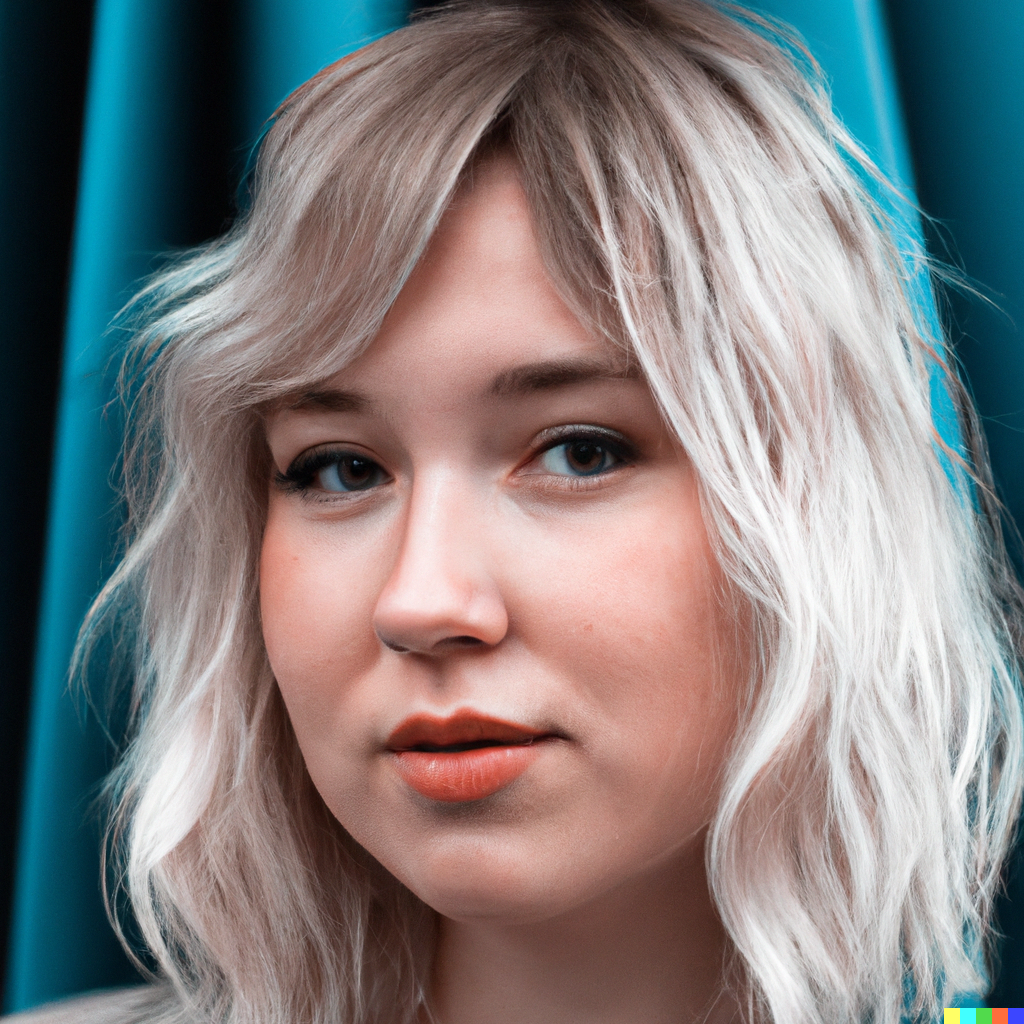
\includegraphics[scale=0.10]{zena.jpg}
\end{center}
\caption{Žena}
\label{fig:zena}
\end{figure}
\newpage

Neki od zanimljivijih nemogućih slika su: “Hamburger u obliku Rubikove kocke, profesionalno fotografisanje hrane” (slika \ref{fig:hamburger}.), “Plišani medvedi rade na novom istraživanju veštačke inteligencije na Mesecu 1980-ih” (slika \ref{fig:medvedi}.)...

\begin{figure}[h!]
\begin{center}
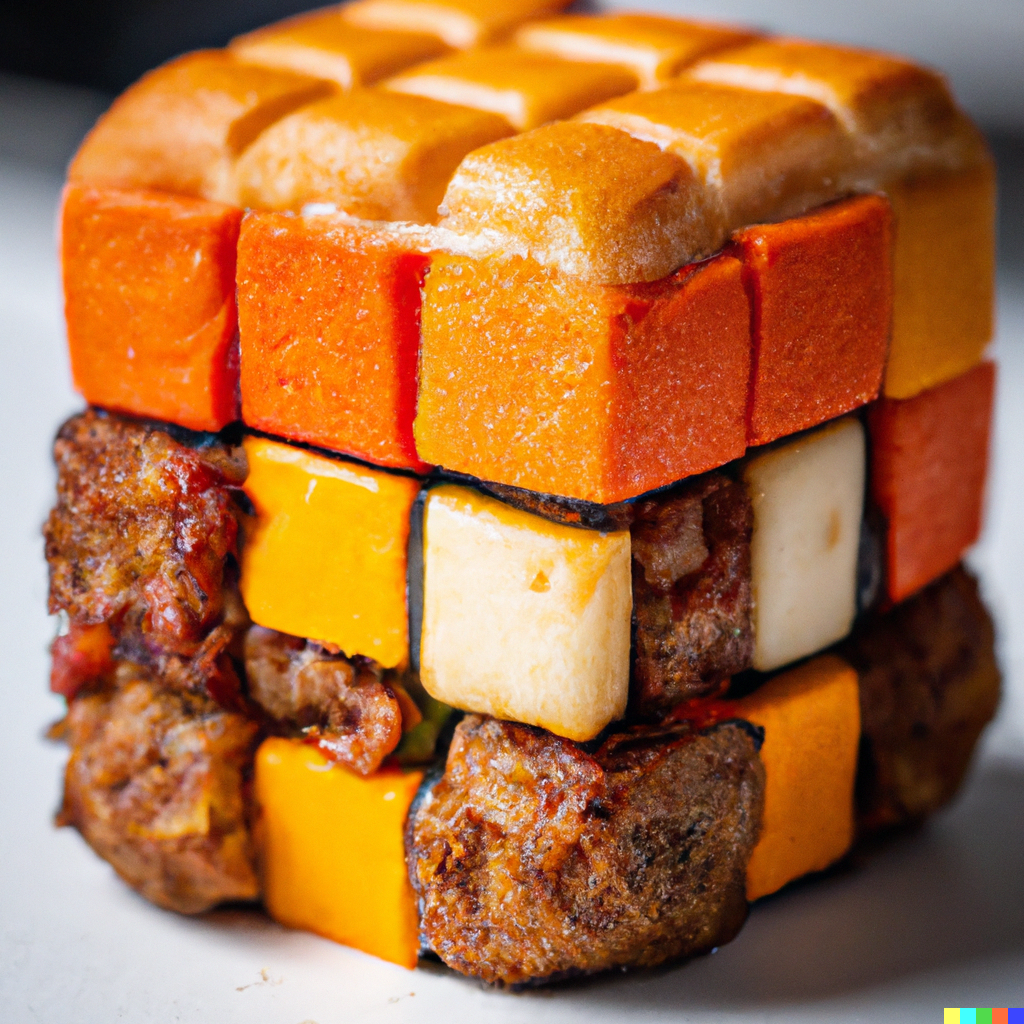
\includegraphics[scale=0.10]{hamburger.jpg}
\end{center}
\caption{Rubikova kocka kao hamburger}
\label{fig:hamburger}
\end{figure}

\begin{figure}[h!]
\begin{center}
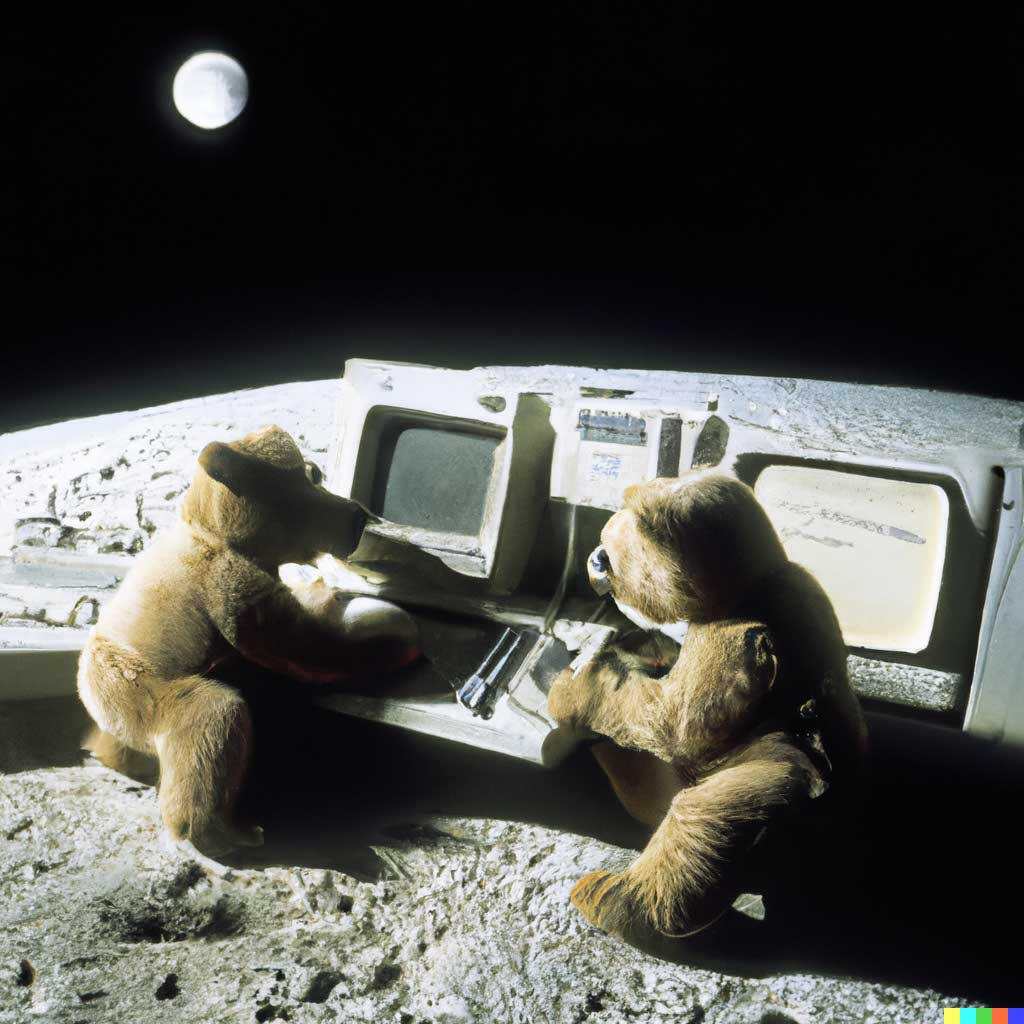
\includegraphics[scale=0.10]{medvedi.jpg}
\end{center}
\caption{Medvedi u svemiru}
\label{fig:medvedi}
\end{figure}


\end{nesto1}
\newpage
\subsection{Etički problemi}
\label{subsec: Etički problemi}
Oslanjanje DALL-E 2 na javne skupove podataka utiče na njegove rezultate i dovodi do algoritamske pristrasnosti u nekim slučajevima, kao što je generisanje većeg broja muškaraca nego žena za zahteve koji ne pominju pol. Podaci o obuci DALL-E 2 su filtrirani kako bi se uklonile nasilne i seksualne slike, ali je utvrđeno da to povećava pristrasnost u nekim slučajevima, kao što je smanjenje učestalosti generisanja žena. OpenAI pretpostavlja da je to možda zato što je veća verovatnoća da će žene biti seksualizovane u podacima o obuci, što je uzrokovalo da filter utiče na rezultate. U septembru 2022., OpenAI je potvrdio za The Verge da DALL-E nevidljivo ubacuje fraze u korisničke upite kako bi se pozabavio pristrasnošću u rezultatima; na primer, „crnac“ i „azijska žena“ se ubacuju u upite koji ne navode pol ili rasu.

Zabrinutost u vezi sa DALL-E 2 i sličnim modelima za generisanje slika je da bi se oni mogli koristiti za propagiranje dubokih fejkova\footnote{Dezinformacije putem slika.} i drugih oblika dezinformacija. Kao pokušaj da se ovo ublaži, softver odbija upite koji uključuju javne ličnosti i rezultate koji sadrže ljudska lica. Upiti koji sadrže potencijalno nepoželjan sadržaj se blokiraju, a otpremljene slike se analiziraju kako bi se otkrio uvredljiv materijal. Nedostatak filtriranja zasnovanog na upitu je to što ga je lako zaobići upotrebom alternativnih fraza  koje rezultiraju sličnim izlazom. Na primer, reč „krv“ je filtrirana, ali „kečap“ i „crvena tečnost“ nisu, pa korisnici na taj način mogu dobiti sličnu sliku izbegavši filtriranje\cite{4}.

Još jedna zabrinutost u vezi sa DALLE-2 i sličnim modelima je da bi mogli da izazovu tehnološku  nezaposlenost za umetnike, fotografe i grafičke dizajnere zbog svoje tačnosti i popularnosti.
\subsection{Tehnička ograničenja}
\label{subsec: Tehnička ograničenja}
Razumevanje jezika DALL-E 2 ima ograničenja. Ponekad nije u stanju da razlikuje žutu knjigu i crvenu vazu od crvene knjige i žute vaze ili pandu koja pravi latte art od late umetnosti pande. Generiše slike astronauta koji jaše konja kada mu se prikaže upit konja koji jaše astronauta. Tako de ne uspeva da generiše ispravne slike u različitim okolnostima. Zahtevanje više od 3 objekta, negacija, brojevi i povezane rečenice mogu dovesti do grešaka i karakteristike objekta mogu se pojaviti na pogrešnom objektu. Dodatna ograničenja uključuju rukovanje tekstom – koji, čak i sa čitljivim slovima, gotovo uvek ispadne kao besmislica u obliku snova– i njegov ograničeni kapacitet da se bavi naučnim informacijama, kao što su astronomija ili medicinske slike.
\newpage
\section{Zaključak}
Ovo je tek početak razvitka veštačke inteligencije, a njene mogućnosti nemaju granice. DALL-E je jedan od najpopularnijih i najpristupačnijih generatora iz teksta u sliku. Pored mnogobrojnih benefita koje DALL-E 2 pruža, postoje i neke loše strane, o kojima treba voditi računa. Ovaj generator dostupan je svima, samim tim i njegova zloupotreba je česta. Korišćenje veštačke inteligencije olakšaće mnoge poslove, a neke poslove čak više ljudi neć ni morati da rade, već će sve moći da se prepusti veštačkoj inteligenciji. Već su mnogi umetnici izgubili svoje poslove jer postoje softveri za generisanje slika (DALL-E 2). 

DALL-E 2 je softver koji predstavlja minijaturnu primenu veštačke inteligencije i pokazuje koliko ona može biti fascinantna i zastrašujuća samo gledajući obične slike. Veštačka inteligencija je oblast koja je u velikom usponu i naš zadatak je da je iskoristimo u humane svrhe i što manje zloupotrebimo.



\addcontentsline{toc}{section}{Literatura}
\appendix


\iffalse
 
\bibliographystyle{plain}
\fi

\begin{thebibliography}{9}

\bibitem{1} Allyn, Bobby. \emph{ Surreal or too real? Breathtaking AI tool DALL-E takes its images to a bigger stage}. NPR. Retrieved 20 July 2022.

\bibitem{2}  OpenAI \emph{  DALL·E 2 Preview - Risks and Limitations}, 19 June 2022 

\bibitem{3}  Macaulay, Thomas \emph{ Say hello to OpenAI's DALL-E, a GPT-3-powered bot that creates weird images from text}. TheNextWeb, 28 January 2021.

\bibitem{4} Sahar Mor, Stripe \emph {"How DALL-E 2 could solve major computer vision challenges"}.

\bibitem{5} Walsh, Bryan \emph{ "A new AI model draws images from text"}


\end{thebibliography}



\appendix





\end{document}
